% \documentclass[aspectratio=169,notes]{beamer}
\documentclass[aspectratio=169]{beamer}
\usetheme[faculty=phil]{fibeamer}
\usepackage{polyglossia}
\setmainlanguage{english} %% main locale instead of `english`, you
%% can typeset the presentation in either Czech or Slovak,
%% respectively.
\setotherlanguages{russian} %% The additional keys allow
%%
%%   \begin{otherlanguage}{czech}   ... \end{otherlanguage}
%%   \begin{otherlanguage}{slovak}  ... \end{otherlanguage}
%%
%% These macros specify information about the presentation
\title[IME]{Introduction to Mechanical Engineering, CAD REN 1} %% that will be typeset on the
\subtitle{Render  
\\ \  
\\ \ 
    } %% title page.
\author{Oleg Bulichev}
%% These additional packages are used within the document:
\usepackage{ragged2e}  % `\justifying` text
\usepackage{booktabs}  % Tables
\usepackage{tabularx}
\usepackage{tikz}      % Diagrams
\usetikzlibrary{calc, shapes, backgrounds}
\usepackage{amsmath, amssymb}
\usepackage{url}       % `\url`s
\usepackage{listings}  % Code listings
% \usepackage{subfigure}
\usepackage{floatrow}
\usepackage{subcaption}
\usepackage{mathtools}
\usepackage{todonotes}
\usepackage{fontspec}
\usepackage{multicol}
\usepackage{pdfpages}
\usepackage{wrapfig}
\usepackage{animate}
\usepackage{booktabs}
\usepackage{multirow}
% \usepackage{graphicx}
\usepackage{colortbl}

\graphicspath{{resources/}}
\frenchspacing

\setbeamertemplate{caption}[numbered]
\usetikzlibrary{graphs}

% \usepackage[backend=biber,style=ieee,autocite=footnote]{biblatex}
% \addbibresource{biblio.bib}
% \DefineBibliographyStrings{english}{%
%   bibliography = {References},}

\newcommand{\oleg}[2][] {\todo[color=red, #1] {OLEG:\\ #2}}
\newcommand{\fbckg}[1]{\usebackgroundtemplate{\includegraphics[width=\paperwidth]{#1}}}%frame background

\usepackage[framemethod=TikZ]{mdframed}
\newcommand{\dbox}[1]{
\begin{mdframed}[roundcorner=3pt, backgroundcolor=yellow, linewidth=0]
\vspace{1mm}
{#1}
\vspace{1mm}
\end{mdframed}
}

\begin{document}
\setlength{\abovedisplayskip}{0pt}
\setlength{\belowdisplayskip}{0pt}
\setlength{\abovedisplayshortskip}{0pt}
\setlength{\belowdisplayshortskip}{0pt}

\fbckg{fibeamer/figs/title_page.png}
\frame[c]{\setcounter{framenumber}{0}
    \usebeamerfont{title}%
    \usebeamercolor[fg]{title}%
    \begin{minipage}[b][6.5\baselineskip][b]{\textwidth}%
        \textcolor{black}{\raggedright\inserttitle}
    \end{minipage}
    % \vskip-1.5\baselineskip

    \usebeamerfont{subtitle}%
    \usebeamercolor[fg]{framesubtitle}%
    \begin{minipage}[b][3\baselineskip][b]{\textwidth}
        \raggedright%
        \insertsubtitle%
    \end{minipage}
    \vskip.25\baselineskip
}
%   \frame[c]{\maketitle}

\fbckg{fibeamer/figs/common.png}

\note{\scriptsize
}



\begin{frame}[t]{Plan}
\framesubtitle{}
\begin{enumerate}
    \scriptsize
    \item What do we want to achieve with the renderer?
    \item CAD vs Polygonal
    \item What defines the material
    \item How to make a photorealistic rendering.
    \begin{enumerate}
        \item How do we make sure we don't mess up the materials?
        \item How do I adjust the scene?
        \item How to set up a light, 3-point lightning?
    \end{enumerate}
    \item How to make it look nice. 
    \begin{enumerate}
        \item Composition
        \begin{enumerate}
            \item Guiding lines
            \item Shape silhouettes
            \item Color/brightness highlighting
        \end{enumerate}
        \item Color balance, brightness
    \end{enumerate}
\end{enumerate}
\end{frame}

\begin{frame}[t]{What do we want to achieve with the renderer?}
\framesubtitle{}
    \centering \LARGE A nice picture showing the result of the IRL will look like.

    \begin{figure}[H]
        \centering
\includegraphics[height=4cm,width=1\textwidth,keepaspectratio]{why.png}
        \label{fig:why.png}
    \end{figure}

\end{frame}

\usebackgroundtemplate{}
\setbeamercolor{background canvas}{bg=}
\includepdf[pages=-,fitpaper, linktodoc=true, pagecommand={\section{Mam_Render}\label{pdf:Mam_Render}}]{Mam_Render.pdf}
\fbckg{fibeamer/figs/common.png}

\begin{frame}[t]{How to make it look nice}
    \framesubtitle{Video}
    \vspace{-0.6cm}
    \begin{figure}[H]
        \href{https://youtu.be/hUmZldt0DTg}{
            \centering
\includegraphics[height=6cm,width=1\textwidth,keepaspectratio]{filmcomposition_video.jpg}}
        \label{fig:filmcomposition_video.jpg}
    \end{figure}
\end{frame}

\begin{frame}[t]{Color balance}
    \framesubtitle{Video}
    \vspace{-0.6cm}
    \begin{figure}[H]
        \href{https://youtu.be/UWwNIMHFdW4}{
            \centering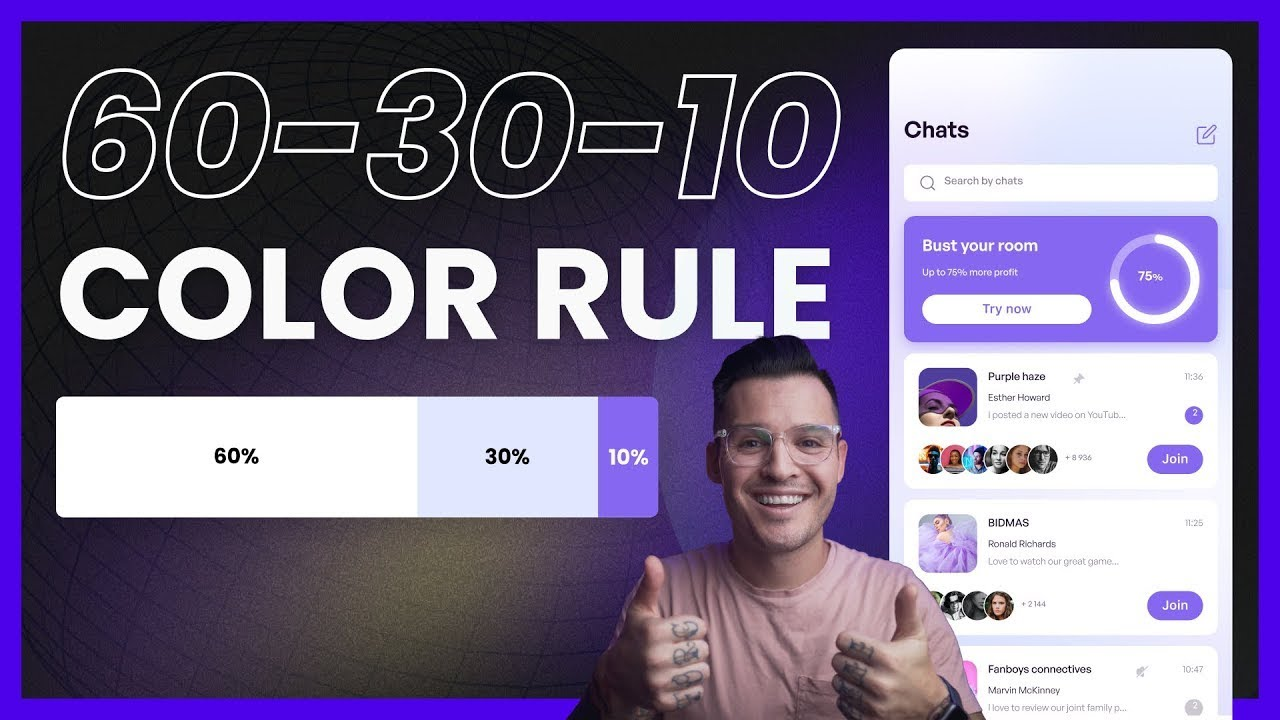
\includegraphics[height=6cm,width=1\textwidth,keepaspectratio]{color_video.jpg}}
        \label{fig:color_video.jpg}
    \end{figure}
\end{frame}

\begin{frame}[t]{NX aspects (ENG)}
    \framesubtitle{}
    \begin{columns}[T,onlytextwidth]
        \begin{column}{0.69\textwidth}
            \begin{itemize}
                \scriptsize
                \item The standard scene is good, the light is already well set up there, and that's the most important thing. What's lacking is a bit more down-to-earth, so we'll take one of the standard scenes (the picture) and go for it.
                \item Metals from the folder Metals - too perfect. Suitable either for slices or for satellites only from the conveyor. For the rest it's better to use variations from the folder Metals-Brushed. Although there they are exactly machined, but they look closer to what we are familiar with IRL.
                \item Chamfers. A mouthpiece is not enough to fully convey how important smoothing the corners is for an adequate looking picture. If the corner is not a blade, then give it at least a millimeter chamfer. It will look a level better.
            \end{itemize}
        \end{column}
        \begin{column}{0.29\textwidth}
            \begin{figure}[H]
                \centering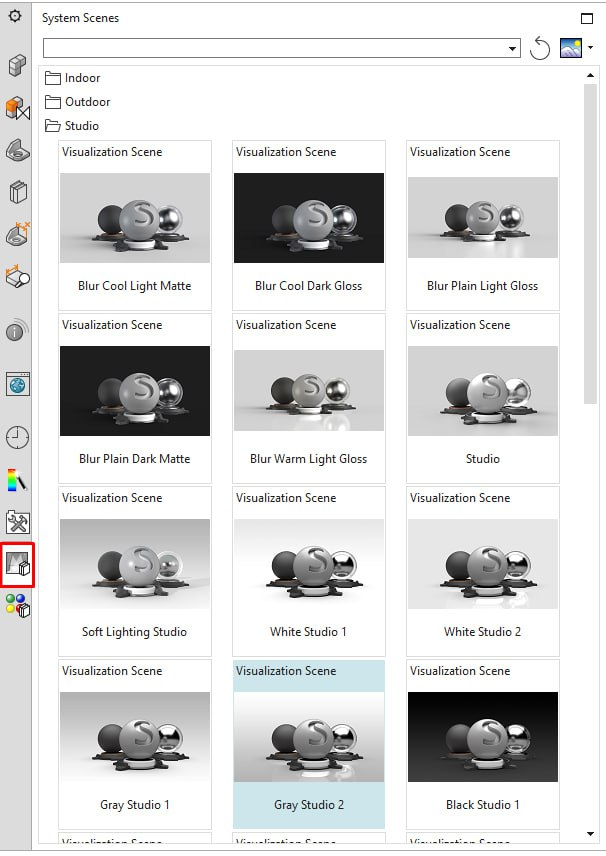
\includegraphics[height=5.5cm,width=1\textwidth,keepaspectratio]{standard_scence.jpg}
                % \caption{caption_name}
                \label{fig:standard_scence.jpg}
            \end{figure}
        \end{column}
    \end{columns}
    \end{frame}
\begin{frame}[t]{NX aspects (RUS)}
\framesubtitle{}
\begin{columns}[T,onlytextwidth]
    \begin{column}{0.69\textwidth}
        \begin{itemize}
            \scriptsize
            \item Стандартная сцена хороша, там свет уже хорошо настроен, а это самое главное. Не хватает приземлённости, для этого выбираем одну из стандартных сцен (картинка) и радуемся
            \item Металлы из папки Metals - слишком идеальные. Подойдут либо для срезов, либо для спутников только с конвеера. Для остального лучше использовать вариации из папки Metals-Brushed. Хотя там они именно обработаны, но выглядят более приближенно к тому что нам знакомо ИРЛ.
            \item ФАСКИ. Капса не хватит что бы в полной мере передать насколько важно сглаживание углов для адекватно выглядящей картинки. Если угол не является лезвием, то дайте ему хотя бы миллиметровую фаску. Выглядеть станет на уровень лучше.
        \end{itemize}
    \end{column}
    \begin{column}{0.29\textwidth}
        \begin{figure}[H]
            \centering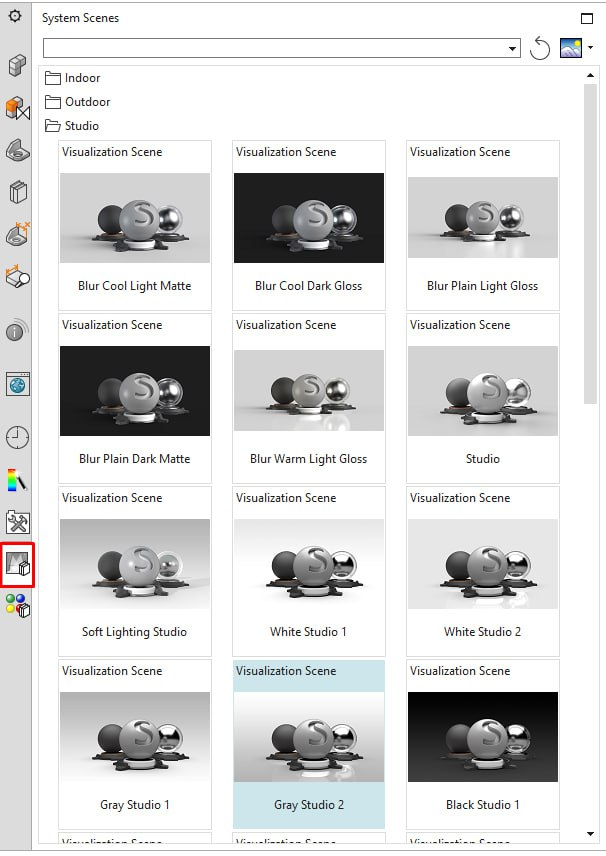
\includegraphics[height=5.5cm,width=1\textwidth,keepaspectratio]{standard_scence.jpg}
            % \caption{caption_name}
            \label{fig:standard_scence.jpg}
        \end{figure}
    \end{column}
\end{columns}
\end{frame}

\begin{frame}[t]{NX Ray Traced Studio material}
\framesubtitle{}
    \begin{enumerate}
        \item \href{https://youtu.be/uyGHuxEY5Gk}{How to use NX Ray Traced Studio}
        \item \href{https://docs.sw.siemens.com/en-US/doc/209349590/PL20200605195244930.viewing_rendering/xid1219739}{Rendering (docs)}
        \item \href{https://youtu.be/qPT449FupKU}{Case study}
    \end{enumerate}
\end{frame}

\begin{frame}[t]{Practical Task: Repeat the video}
    \framesubtitle{Video}
    \vspace{-0.6cm}
    \begin{figure}[H]
        \href{https://disk.yandex.ru/i/aXWXryrDGGdZ0A}{
            \centering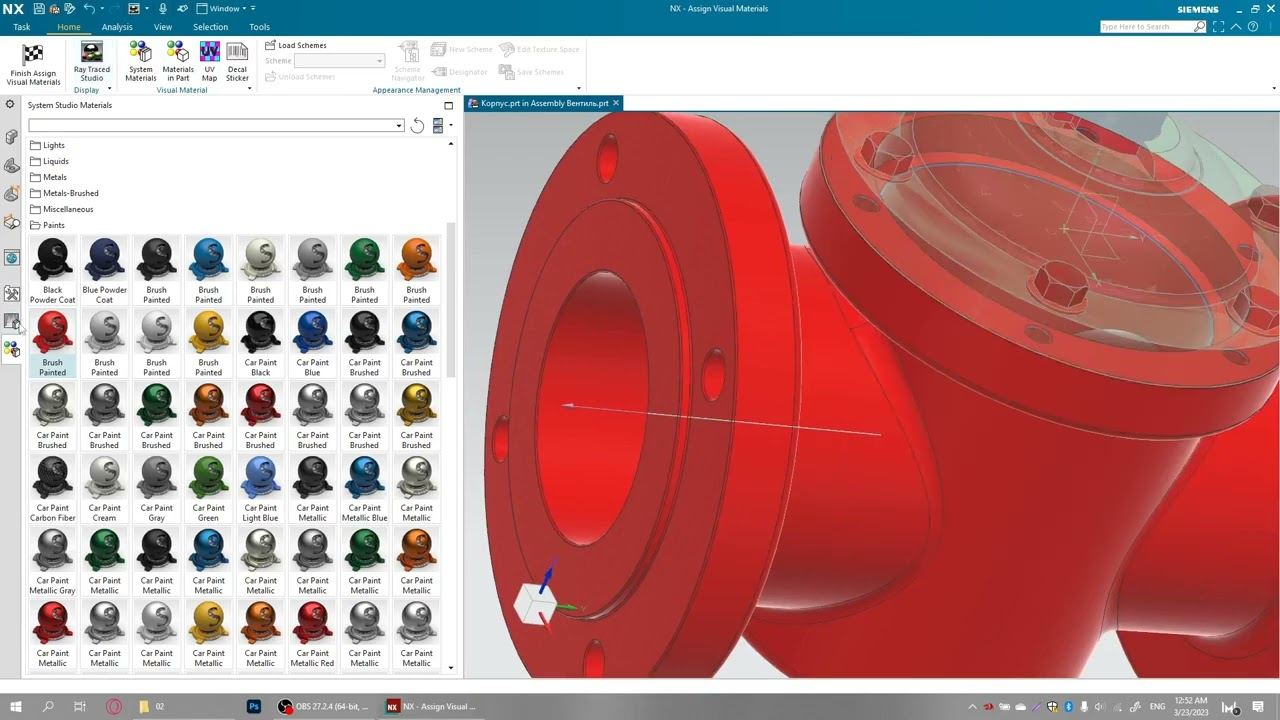
\includegraphics[height=6cm,width=1\textwidth,keepaspectratio]{practice_render.jpg}}
        \label{fig:practice_render.jpg}
    \end{figure}
\end{frame}

\begin{frame}[t]{Invited Lecturer Egor (RUS)}
    \framesubtitle{Video}
    \vspace{-0.6cm}
    \begin{figure}[H]
        \href{https://disk.yandex.ru/i/g4k_bOkkXyebJA}{
            \centering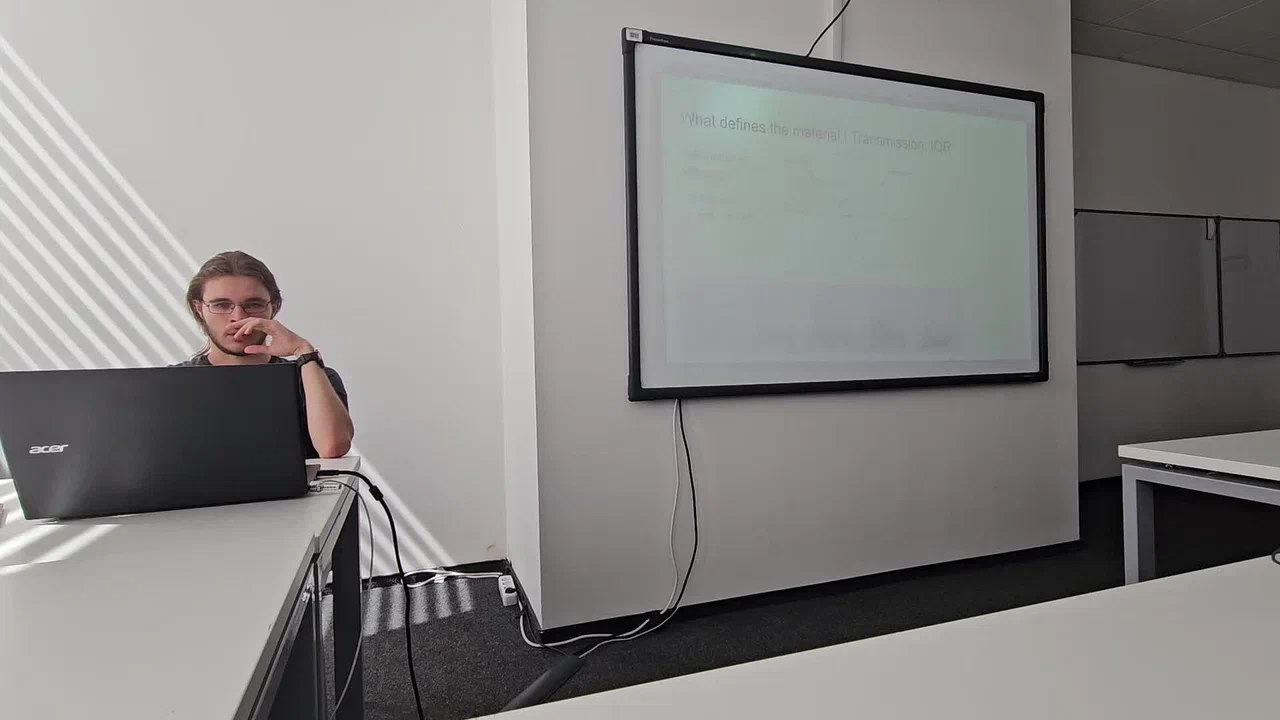
\includegraphics[height=6cm,width=1\textwidth,keepaspectratio]{egor_render_video.png}}
        \label{fig:egor_render_video.png}
    \end{figure}
\end{frame}

% \begin{frame}[t]{Reference Material}
% \framesubtitle{}
% \footnotesize
% \begin{enumerate}
%     \item \ 
% \end{enumerate}
    
% \end{frame}

\fbckg{fibeamer/figs/last_page.png}
\frame[plain]{}

\end{document}